\chapter{Variational Autoencoder} \label{genmod}
\section{Introducing the problem}



\section{Generative Models Overview}

Generative models are a class of machine learning algorithms that aim to learn distributions $P(X)$ over a dataset $X | x \in \mathcal{R}^\mathcal{D}$. The class of generative models approach pattern recognition in line with Feynman's "what I cannot create I do not understand". Given a point $x \in X$ a generative model will try to uncover the patterns existing in $x$'s structure, i.e. between the parts that comprise $x$, and often, this learnt space that describes the patterns inherent in the structure of $X$ is low-dimensional.\\

Generative models generally fall under the umbrella of unsupervised learning, and often have applications similar to those of other traditional unsupervised learning methods such as PCA, Gaussian-Mixture-Models and Kernel Density Estimation. When tasked with uncovering a distribution $P(X)$ over a dataset $X$ these generative models can be used to uncover the density distribution over the dataset, and consequently allow us to measure things like the likelihood of points in this space, similar to GMMs and KDE. When tasked with learning a distribution $P(Z)$ that is generative of $X$ where $dim(z) < dim(x)$ then effectively these generative models learn a lesser-dimensional space that minimises some measure of reconstruction error, similar to PCA and Kernel-PCA.\\

Beyond learning distributions $P(X)$ and $P(Z)$ over the dataset, generative models also allow us to sample points from the learned distribution. For example, by learning a distribution over a dataset of images of trees, a generative model will allow us to sample new images of trees from the distribution that look very much like the images in our database, but aren't exactly like the images we already have. One can imagine the applications of this in graphic design and video production! Training models that allow us to generate completely new samples from the learned distribution have been explored for quite some time in the machine learning community, however until recently they have all faced one of three problems: they make strong assumptions about the structure in the data, and when these assumptions do not hold, they make sub-optimal approximations that fail to comprehensively learn generative distributions. When the models succumb to neither of these shortcomings, they often rely on very expensive inference techniques like Markov Chain Monte Carlo \citep{doersch2016tutorial}.\\

Recently, two new classes of generative models have emerged that address all three of these problems: Generative Adversarial Networks \citep{goodfellow2014generative} and the Variational Autoencoder \citep{kingma2013auto}. Generative Adversarial Networks operate within the framework of finding a Nash Equilibrium between a generator network, $G$ that learns the distribution $P(X)$ and a discriminator network $D$ that attempts to classify whether the points generated by $G$ do come from the space inhabited by the data points. Variational Autoencoders on the other hand have sprung out from the merger of Bayesian inference with Machine Learning, particularly the Autoencoder. In this chapter, we will explore the Variational Autoencoder and its application to estimating a distribution over our dataset, and in the process uncovering the structure and patterns in the way user's truly use their applications.


\section{Variational Autoencoder}
\subsection{Autoencoder}
Traditional Autoencoders behave like compression-decompression algorithms in that they take high dimensional data and embed them into a low dimensional space, and from that space they attempt to reconstruct the original input. In doing so, Autoencoders are trained to minimize the reconstruction error by finding a hidden representation that accounts for as much of the variance as possible. In that sense, they behave most similarly to PCA. The process of training a model that learns this encoding-decoding process is normally known as representation learning. The benefits of these models normally stem from the myriad ways these low-dimensional representations can be used. For example, they can be used to learn similarities between objects based on distances in this lower dimensional space, for use in NLP systems in semantic embedding, or for reducing the dimensionality of inputs to other models.

 \begin{figure}[htbp]
     \centering
     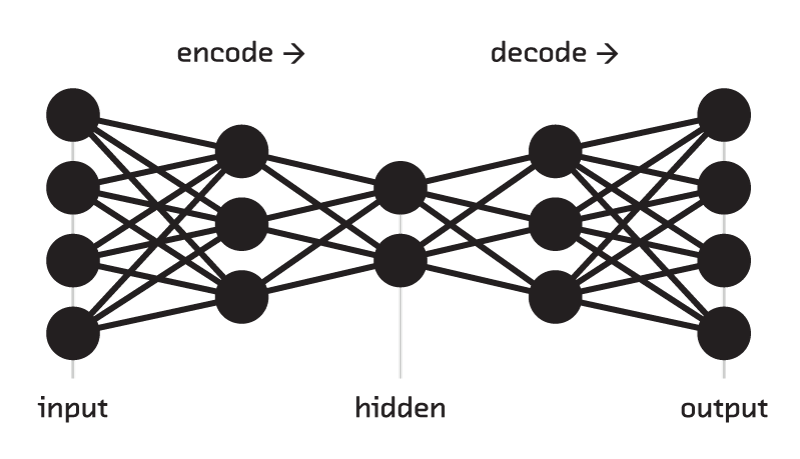
\includegraphics[width=1\textwidth]{images/miriams-figure.png}
     \caption{Autoencoder, \citep{_lorenz_}}
     \label{fig:ae}
 \end{figure}
 
 This process of training only on the reconstruction error often results in learning low-dimensional mappings that minimise information loss, behaving very similarly to other dimensionality reduction techniques like PCA. When trained as such, the Autoencoder consequently doesn't learn any new and interesting features about the dataset it is encoding. To remedy this, many interesting advances have been made in regularising the Autoencoder. At the cost of fidelity, regularisation, for example enforcing sparsity constraints and regularising the weights of the encoder/decoder, forces the Autoencoder to discard all but the most salient and important hidden features. The Variational Autoencoder is a form of Autoencoder that regularises the encoding-decoding process by simultaneously learning a distribution over the data and over a latent space with a designated prior.
 
\section{Variational Autoencoders}

\subsection{Intuition} \label{vae_intuition}
Consider the task of generating images of animals. When people generate images, for example by drawing or just plain imagination, we make a set of decisions before generating the image. To generate the image of a dog, we first decide what it is we wish to generate, the first obviously being that what we wish to generate is the image of a dog and not a cat. Next we might decide that the dog we wish to generate an image of is a Dalmatian. By deciding that the dog will be a Dalmatian we have implicitly made other decision about this dog: that it will be short-haired and spotted. This is an example of the dependencies present in real-world data that are not accounted for by models like Autoencoders. Next, we may decide that this dog will be quite a large dog. In doing so our image of the large Dalmatian dog is constrained by the normal proportions existent in Dalmatian dogs. We cannot have a large Dalmatian with a head the size of a pebble, or feet the size of an elephant's. These decisions illustrate a key characteristic about the process of generating realistic images of animals: before generating anything, we first make a decision about what animal we want to generate an image of. Next we decide on the properties of this animal. In order for the image to be realistic the properties we decide on must be constrained and they must respect the dependencies between different properties of the respective animal, i.e. a Dalmatian's body has certain proportions it must respect be it a large or small Dalmatian. Formally speaking, before generating an image we make a set of decisions on what latent variables our image will be generated from \citep{doersch2016tutorial}, subject to constrains on the dependence of different latent variables on each other.\\

\subsection{Theory} \label{vae_theory}
The process discussed in \ref{vae_intuition} illustrates the concept of a latent variable model. Variational Autoencoders make the assumption that an observation $x \in X$ is just the tip of the iceberg. $x$, in fact, is just a sample that is generated from $z$, a variable in a hidden/latent space $Z$.

 \begin{figure}[htbp]
     \centering
     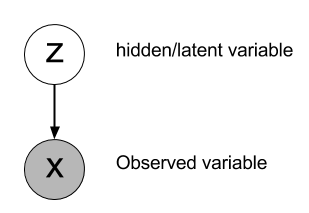
\includegraphics[width=0.5\textwidth]{images/latent.png}
     \caption{Latent variable, from \citep{eric_jang}}
     \label{fig:latent}
 \end{figure}

Given this setup, assume we have a distribution $P(z)$ over $z$ from which we can easily sample points, and that $x$ is generated by mapping a sample $z$ from the latent space to $X$ by a deterministic function $f(z;\theta)$ which is parameterised by some vector $\theta$ from another space $\Theta$. To learn a generative model we would therefore want to learn a $f(z;\theta)$ that creates $x$'s that are likely under $P(X)$. If we do learn such an $f(z;\theta)$ we expect its outputs to follow the distribution $\mathcal{N}(X|f(x;z), \sigma^2 * I$. This simply means that our function $f$ creates points that are likely to produce samples that are like $X$ and not produce samples that are not like $X$. Now, if we want to generate points that are realistic, i.e. likely, then we wish to maximise, under the generative process and training set, the probability $P(X)$. Using the law of total probability, we can set up this problem as maximising the following

\begin{equation}
    P(X) = \int P(X|z;\theta)P(z)dz
\end{equation}
where we have marginalised $z$ out of $P(X,z)$ and $P(X|z; \theta)$ replaces $f(z;\theta)$. Formulated like this, it becomes straightforward to estimate $P(X)$, all we have to do is sample points $N$ latent variables $z$ from $P(Z)$ and estimate $P(X)$ as follows:

\begin{equation}
    P(X) = \frac{1}{N} \sum_i^N P(X|z_i)
\end{equation}

To sample $z_i$'s from $P(z)$ we would need to know what the distribution of $P(z)$ is, which we don't. The VAE addresses this by observing that whatever the distribution of $P(z)$ is, if it is $d$ dimensional then it can be approximated by $d$ normally distributed random variables and a sufficiently complex function approximator, which we already have in $f(z;\theta)$! The process of generating $X = f(z; \theta)$ now becomes a two-step process where we first sample $z$ from a standard normal $\mathcal{N}(0,1)$, then mapp this sampled $z$ to the true latent, which we now rename to $\hat{z}$, from which we finally generate $X$. Normally, $f(z;\theta)$ is modelled by a sufficiently high capacity neural network to ensure it is capable of learning the mapping from $z$ to $\hat{z}$ to finally $X$.\\

Now that we have a way of sampling $z_i$, computing $\frac{1}{N} \sum_i^N P(X|z_i)$ becomes possible once again. However, given that we have defined $z_i$ to come from $\mathcal{N}(0,1)$ and observing that $P(z|X)$, the subspace of $P(z)$ that is likely to have generated $X$, is likely substantially smaller than $P(z)$ we note that in practice we would require many samples of $z_i$ for $P(X|z_i)$ to sufficiently approximate $P(X)$. The process of sampling many points from $P(z)$ results in very slow convergence is undesirable. Ideally, it would be preferable if we only sampled $z_i$'s from $P(z)$ that are likely to have generated $X$, i.e. from $P(z|X)$ however this posterior is usually intractable to compute. Instead of trying to infer this intractable posterior, the VAE performs inference on another distribution $Q(z|X)$ which is chosen to follow a distribution we know how to perform inference over, normally a Gaussian $\mathcal{N}(z|\mu_q(X), \sigma_q(X)$. The mean $\mu_q(X)$ and standard deviation $\sigma_q(X)$ are created through some deterministic sufficiently complex function approximator, for example a neural network, $g(X;\phi)$ in a similar fashion to $f(z;\theta)$. The trick is to realize that while $Q(z|X)$ is not the same as the true $P(z|X)$, if we manage to find a $Q(z|X)$ that is similar to $P(z|X)$ through, for example, mean-field approximation, then our sampled points $z_i$ would be good enough.

 \begin{figure}[htbp]
     \centering
     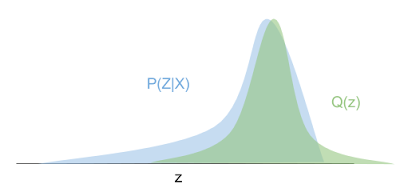
\includegraphics[width=0.5\textwidth]{images/mean-field.png}
     \caption{Q(z): a variational approximation to P(z|X) \citep{eric_jang}}
     \label{fig:mean_field}
 \end{figure}

Mean-field Variational Bayes defines the Reverse KL Divergence as an appropriate measure of dissimilarity between two distributions. To achieve a $Q(z|X)$ that resembles $P(z|X)$ we would like to minimize this KL-Divergence metric:

\begin{equation}
    KL(Q(z|X)||P(z|X)) = E[\log Q(z|X) - \log P(z|X)]
\end{equation}

By applying Bayes' rule to $P(z|X)$, and rearranging the above we arrive at:

\begin{equation} 
    KL(Q(z|X) || P(z|X)) = E[\log Q(z|X) - \log P(z)] + E[\log P(X|z)] + \log P(X)
\end{equation}

Here, we make two observations:

\begin{itemize}
    \item The term $E[\log Q(z|X) - \log P(z)]$ is nothing but the KL-Divergence between $Q(z|X)$ and $P(z)$. Given that we defined $P(z)$ to be $\mathcal{N}(0,1)$ and $Q(z|X)$ to be $\mathcal{N}(z|\mu_q(X), \sigma_q(X)$ this becomes a KL-divergence between two multi-variate Gaussians (with a k-dimensional Gaussian) which has a closed form solution:
    \begin{equation}
        KL (Q(z|X), P(z)) = \frac{1}{2} (\sum_k (\sigma_q(X) + \mu_q^2(X)^T - 1 - \log (\sigma_q(X))
    \end{equation}
    \item The term $E[\log P(X|z)]$ is the reconstruction error between generated points $X$ from our latent space $z$
\end{itemize}
 
 and, after rearranging, finally state the Variational Autoencoder Loss:
 \begin{equation}
      \log P(X) - KL(Q(z|X) || P(z|X)) =  KL (Q(z|X), P(z)) + E[\log P(X|z)]
 \end{equation}
 
 This loss function has an intuitive meaning: we learn our model's distribution $\log P(X)$ subject to some error $KL(Q(z|X) || P(z|X))$ by minimising the reconstruction loss of of our generator $\log P(X|z)$ and the divergence of the latent space produced by our encoder $Q(z|X)$ from the prior on the latent space $P(z)$. It also neatly summarises how a VAE is trained: To learn the distribution $P(X)$, the VAE's Encoder $g(X; \phi)$ learns how to transform $X$ into the latent space $z$ such that the distribution $Q(z|X)$ is as close as possible to the true $P(z)$. Next, the decoder samples points from $Q(z|X)$ and decodes them back into the original space $X$ and is trained to minimize this reconstruction error. The VAE can be trained end-to-end using Stochastic Gradient Descent (SGD) albeit for one problem: while SGD can handle stochastic inputs, it cannot backpropagate errors through stochastic variables like the sampled values of $z$. To overcome this, VAE's employ the \textit{reparameterization trick} whereby instead of sampling $z$ from $\mathcal{N}(\mu_q(X), \sigma_q(X))$ it is sampled from $\mu_q(X) + \epsilon*\sigma_q(X)$ where $\epsilon \in \mathcal{N}(0,1)$. By doing this, we can push $\epsilon$ out of the network to become a stochastic input which SGD can handle. This makes the entire network differentiable end-to-end and trainable by SGD. A schematic of the VAE is shown in Figure \ref{fig:vae_schema}.
 
 \begin{figure}[htbp]
     \centering
     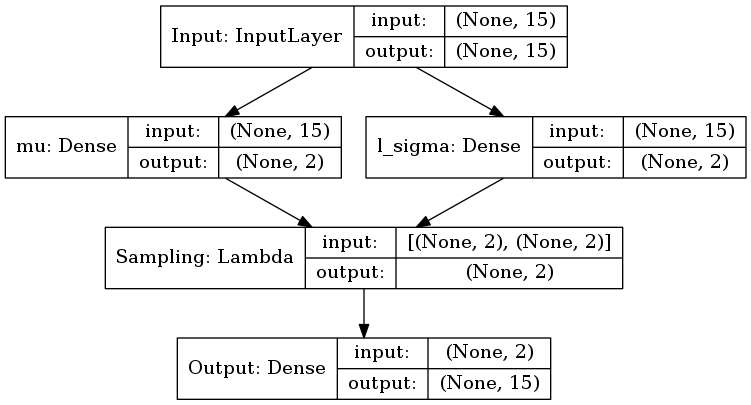
\includegraphics[width=0.5\textwidth]{images/vae}
     \caption{Schema of Variational Autoencoder}
     \label{fig:vae_schema}
 \end{figure}

\section{Implementation \& Results}
In many applications of machine learning, dimensionality reduction is performed prior to training models. By reducing the dimensionality of the input space we strive to make the learning task easier by reducing the amount of information the model has to learn about the input space. While this particularly applies to tasks where the input space is very high-dimensional that it results in very large models, that need not be the case. Often times, the input to our model can be low-dimensional but sparse, or noisy, or both at the same time. In other cases, the data might be simultaneously highly-structured and be highly varied. To give a concrete example, let us consider our own dataset of app-usage behaviour. More specifically, let us consider a particular task our user regularly engages in: Software Development. Given that our data points are aggregated points over 5-minute blocks, each 5-minute block where the user is 'focusing' on Software Development can be highly-varied. In certain cases the user might be testing their program and thus visualising a lot of the results. The user may use various different apps to visualise their results. They might also be consulting online forums and Github for support developing her program. At different times the user may be utilising any number of these different apps to perform the same task of Software Development. Even further, given the same set of apps used in different time steps, the distribution of time across these applications may vary highly as they are subject to many events which we cannot account for in our models. We can choose to consider these external factors on which the particularities depend and that we cannot model as 'noise'. \\

Given such a dataset, it may be helpful to use a dimensionality-reduction procedure that captures these main modes of operation and reduces the variance in the model. A particularly common algorithm used for this purpose is Principal Component Analysis. Alternatively, a Variational Autoencoder's encoder can be used for the same purpose and in what follows we compare the results of dimensionality reduction on our dataset between PCA and the VAE's encoder. 

\subsection{PCA Results}
Principal Component Analysis is a statistical orthogonal transformation that converts a set of observations comprising possibly correlated features in a space into a subspace where the new features are uncorrelated and explain the maximum variance in the dataset. The results are such that the first principal component explains the maximum variance in the dataset, the second component explains less than the first and so on. To visualise the results of PCA, we apply the transformation to our dataset and, for the sake of visualisation, plot the dataset against the first and second principal components:

\begin{figure}[htbp]
    \centering
    \includegraphics[width=1\textwidth]{images/PCA}
    \caption{Principal Component Analysis}
    \label{fig:pca}
\end{figure}

To describe the plot: each point represents an Activity Vector that describes the distribution of time spent across the activities in $\mathcal{P}$. Each app in $\mathcal{P}$ has a colour associated with it shown in Figure \ref{TimeSpentDistribution}. In this plot, and all plots of the dataset that follow, each point's colour is a weighted sum of the colours of each app, weighted by time spent on the respective app. For example, a point that represents a five minute block in which the user solely does 'Software Development' will have a colour corresponding to that of 'Software Development': orange. In the case where the user uses only Instant Messaging apps, the colour will be the corresponding green. If the user splits their time between these two activities, then the colour of that point will be a weighted average, or blend, between orange and green according to the time spent across the two activities. Also worth noting, the brighter a colour the more time spent on that particular app, and consequently dark points indicate points where the distribution of time across all apps in the 5-minute block does not sum up to 300 seconds. \\

As can be observed from the PCA plot, low-dimensional space into which the datapoints are projected tries to account for the maximum amount of variance in the original dataset by prioritising the apps whose usage varies the most. Intuitively, we can see this from the plot by observing that the points are clustered along 3 main axes: Video, Instant Messaging and Software Development. While some co-occurrence information is captured, for example the set of points between the two main orange and green axes that tells us Software Development and IM tend to happen together, by and large the PCA embeddings discard most of the information that does not explain variance. In datasets where certain features tend to have much larger variance than others, this is expected. Normally, such a problem would be easy to correct for by scaling the features to have the same variance, however this scaling inherently destroys the important information encoded in the scale of variance of different apps. Naturally, the way we use our different applications have unique patterns. Certain classes of apps, like Instant Messaging, are used either sparingly in a 5-minute block, or are focused on entirely and consume the entire 5-minute block. Other apps like search are mostly used sparingly in 5-minute blocks, mostly as a transition stage into other apps (Browser, General News \& Opinion, Reference \& Learning). This difference in usage pattern is an important piece of information we would not wish to discard, and is quite critical in truly understanding how a person uses their applications. This example illustrates the short-coming of PCA's emphasis on variance which make it an inappropriate tool for encoding app-usage data, summarized below:

\begin{itemize}
    \item PCA is scale-invariant and consequently penalises features that have a lesser magnitude of variance.
    \item It is possible to correct for the above by pre-scaling the features to have the same magnitude of variance.
    \item Pre-scaling however destroys the information inherent in the scale of variance across different features.
\end{itemize}

In addition to the suboptimality of encoding to maximise variance in this dataset, PCA makes the assumption $P(X)$, the density distribution over $X$ is a Gaussian distribution. This assumption may not necessarily hold in the case of our dataset, while the individual features may be normally distributed, $P(X)$ may result from a non-linear relationship between the individual components, which inherently cannot be captured by PCA. Ideally, we would like a dimensionality-reduction technique that makes a minimal set of assumptions about the form of $P(X)$, such as the VAE.


\subsection{VAE Encoder Results}
The VAE overcomes the shortcomings of the PCA through the following properties:
\begin{itemize}
    \item The VAE makes no assumptions about the form of $P(X)$. Instead it approximates it using the standard normal $Q(X)$ by minimising the Kullback-Leibler divergence between $P(X)$ and $Q(X)$. By not making any assumptions about $P(X)$ the VAE is not hamstrung by input data that is not normally distributed. In fact, to an extent, the VAE can handle input data that comes from any distribution.
    \item The VAE's loss function tries to jointly minimise the reconstruction error $\log P(X|z)$ and the KL-divergence $KL (Q(z|X), P(z))$ where $P(z)$ is our prior on the density distribution of the latent space.
\end{itemize}
The second point is particularly important in understanding the difference between the VAE's encoding process and PCA. To illustrate this, consider the regular Autoencoder (AE). An AE is also a two-stage encoder-decoder neural network that encodes input data X into a lower dimensionality space H, and decodes from H back to X. The AE is a simpler case of the VAE where there is no stochastic component (sampling) and everything is deterministic. In comparison to the VAE, the AE is trained to solely minimize the reconstruction error. Given a linear AE trained under this objective function, the linear AE will learn to approximate the optimal linear encoder - PCA \citep{Goodfellow-et-al-2016} The VAE moves beyond this by both allowing for non-linear encoders and decoders and regularising the encoding process through enforcing a normal distribution on the latent space. Consequently, during encoding we expect the VAE's encoder to move beyond encoding for maximum variance to learning a more representative encoding, i.e. latent space, of the data. 

 \begin{figure}[htbp]
     \centering
     \includegraphics[width=1\textwidth]{images/VAE_Latent_Space3}
     \caption{Latent space of the VAE's encoder}
     \label{fig:vae_latent}
 \end{figure}

By comparing the plot of the PCA encoding against that of the VAE, we observe that while both plots share a similar feature in how the data is distributed, primarily along different axes on which one particular app is concentrated, the VAE's encoder is able to assign equal important to the different apps, assigning each one a component of variance along which it is dominant. This contrasts with the PCA's encoding where only 3 major axes of variation are represented. A critical point to note is that while indeed the VAE is able to distribute importance more evenly across the different apps, the latent space is still characterised by sparsity in between the major components of variance, on which a single app is dominant. Given the normal distribution prior imposed on $P(z)$, we instead expect to see the distribution of points in the latent space, $Q(z|X)$, following the standard normal prior $\mathcal{N}(0,1)$. Moreover, from Figure \ref{fig:vae_losses} and Table \ref{my-vae_losses_table}, we observe that the majority of the VAE's error comes from the reconstruction component, suggesting that the VAE has a harder time learning the inter-app dependencies.\\

Two possible explanations exist for why the encoder learns such a latent space $Q(z|X)$:

\begin{itemize}
    \item The latent space of the VAE does not suffice to explain all the dependencies in the data. Consequently the VAE chooses to prioritise encoding latent variables that minimize reconstruction error by explaining the maximal intra-app variance.
    \item The failure to capture inter-app dependencies stems from the source data itself. The 5-minute Activity Vectors do not contain enough information that facilitates learning the inter-app dependencies.
\end{itemize}

 \begin{figure}[htbp]
     \centering
     \includegraphics[width=1\textwidth]{images/VAE_Losses}
     \caption{VAE loss vs epochs}
     \label{fig:vae_losses}
 \end{figure}

\begin{table}[htbp]
\centering
\caption{VAE Training and Validation losses}
\label{my-vae_losses_table}
\begin{tabular}{lll}
                     & Training          & Validation        \\
VAE Loss             & 0.3569    & 0.4659    \\
KL-Divergence         & 1.08499e-05 & 3.3512e-06 \\
Reconstruction Error & 0.3569   & 0.4659  
\end{tabular}
\end{table}


\subsubsection{Size of latent space}
Intuitively, one way to enable the VAE's encoder to learn a richer latent variable model is by increasing the size of the latent space, and possibly allowing the VAE to encode more information. To visualise the effect increasing the latent space has on the VAE loss we plot the validation loss vs latent space size in Figure \label{fig:vae_loss}.

 \begin{figure}[htbp]
     \centering
     \includegraphics[width=1\textwidth]{images/VAE_latent_size_loss}
     \caption{VAE loss vs latent space size}
     \label{fig:latent_size}
 \end{figure}

From Figure \ref{fig:latent_size} we observe that increasing the size of the latent space has minimal effect on the VAE loss and in fact, a larger latent space has a slightly deleterious effect on the VAE loss. Upon inspection of Figure \ref{fig:vae_latent} this makes sense as the VAE's latent space spans a minimal subspace of the prior on $P(z)$ and is heavily concentrated around the origin. This hints that the data does not contain sufficient information to merit encoding latent variables that span a large subspace, particularly as centring points near the origin minimises the KL-Divergence maximally.

\subsubsection{Datapoints lack sufficient information}
Given that the constraint on the size of latent space does not obstruct the VAE from learning a richer latent variable model, we hypothesise that the data points themselves do not contain any information about the dependencies between their constituent apps. To test this hypothesis we would need to observe the effect of conditioning the VAE on other factors that supply additional information that could potentially help the VAE learn a richer set of latent variables. Possible external factors that could be important in learning a richer latent variable model are: time of day, day of the week and previous app-distributions, i.e., what apps the user used before the current Activity Vector. One benefit of the VAE architecture is that it allows for the encoding and decoding process to be conditioned on external factors. When conditioned on external factors, the VAE becomes a Conditional Variational Autoencoder (CVAE) \citep{sohn2015learning, doersch2016tutorial}. In the next chapter we introduce the CVAE and examine the results of conditioning on time of day, day of week and on previous app-activity.

\section{Conditional Variational Autoencoder}
\subsection{Theory}
The Conditional Variational Autoencoder is an extension of the VAE that introduces a level of control over the generation process. While the VAE attempts to infer the latent space $Q(z|X)$ by building a latent variable model that tries to describe the fundamental decision necessary to generate data, the CVAE allows us to directly introduce external pre-determined latent variables into the space. To return to the example of generating images of animals we discussed in Section \ref{vae_intuition}: When learning $Q(z|X)$ such that it describes the 'fundamental decisions' that need to be made before an image is generated we have no control over what variables the encoder learns. The CVAE remedies this by allowing us to condition the entire generative process on an external latent variable $c$ to obtain a new latent space $Q(z|X,c)$ \citep{sohn2015learning}. To understand the difference between the VAE and the CVAE let us return to the VAE loss developed in Section \ref{vae_theory}:

\begin{equation}
  \log P(X) - KL(Q(z|X) || P(z|X)) =  KL (Q(z|X), P(z)) + E[\log P(X|z)]
\end{equation}

From the loss function we observe that the encoder learns the distribution $Q(z|X)$ such that it is entirely dependent on $X$ irrespective of what other information there may be about $X$, i.e., it disregards the different \textit{types} of $X$. More specifically, it learns a \textit{unimodal} distribution on $X$ whereas in fact, $X$ may have a \textit{multimodal} distribution! The same situation holds true for the decoder. To transform the VAE into a CVAE the encoder and decoder networks must be modified to allow condition on a random variable $c$. By doing this the CVAE loss function becomes:

\begin{equation}
  \log P(X|c) - KL(Q(z|X,c) || P(z|X,c)) =  KL (Q(z|X,c), P(z|c)) + E[\log P(X|z,c)]
\end{equation}

By conditioning the generative process on the random variable $c$, the CVAE learns a conditional distribution on the latent space $P(z|c)$. This has applications in many fields, particularly in 'hole-filling' \citep{doersch2016tutorial} where a CVAE is trained to fill holes in sequences by conditioning the output on elements to the left and right of the 'hole'. In what follows we explore conditioning the VAE on the Time \& Day of the activity and on the previous activity vectors. For the time condition we only use the hour component as, empirically, that generates better results.

Practically, conditioning a VAE on a variable $c$ is done by concatenating the input to the VAE with the random variable $c$ such that the input to the encoder is $[x,c]$. The encoder then encodes $[x,c]$ into the latent space $Q(z|X,c)$ to obtain the parameters $(\mu_q(X), \sigma_q(X))$ from which it samples a point. During decoding, the condition variable $c$ is once again concatenated with the sampled point to obtain $[z,c]$ which the decoder reconstructs the original input from. 

 \begin{figure}[htbp]
     \centering
     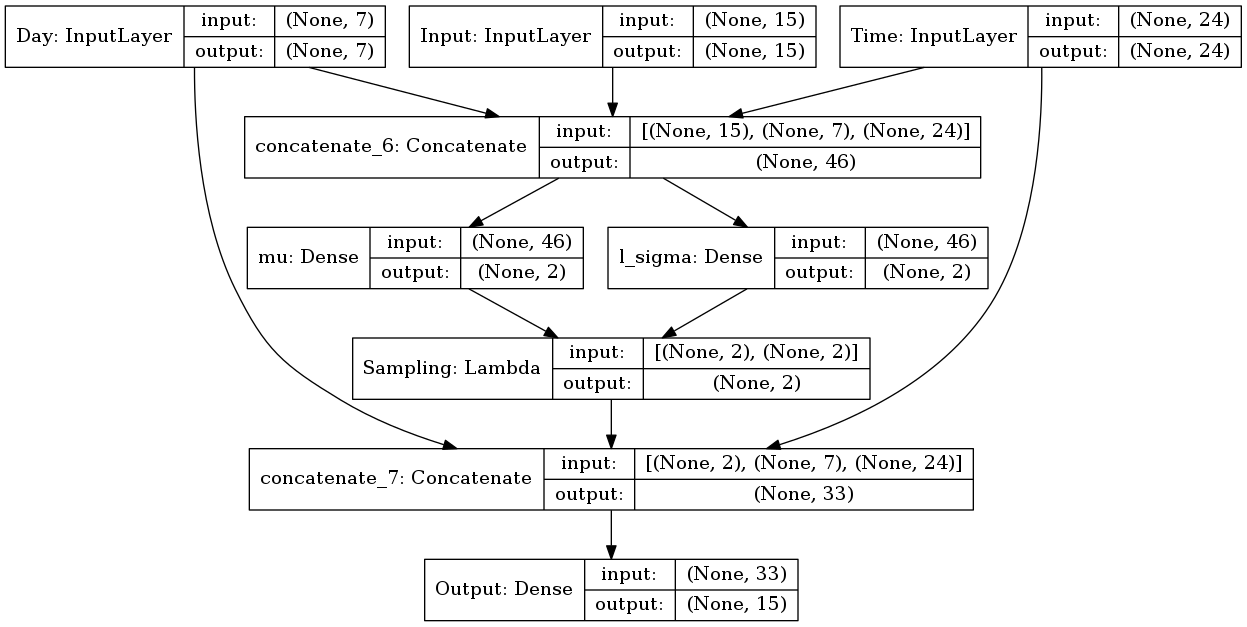
\includegraphics[width=1\textwidth]{images/c_vae}
     \caption{Schema of Conditional Variational Autoencoder}
     \label{fig:cvae_schema}
 \end{figure}
 
\subsection{Intuition}
To understand intuitively what we would expect the CVAE to accomplish, let us consider the case of learning the density distribution $P(X)$ over a dataset $X$ where each $X$ has a label $y$ for each $x \in X$ that tells us explicitly what $x$ is. More specifically, let us consider the case of handwritten digits and the MNIST dataset. When training a VAE to learn the density distribution of the MNIST dataset, we would expect the encoder to learn an encoding $Q(z|X)$ that clearly delineated between the different digits. Intuitively this makes sense since in order to generate different digits the decoder has to 'decide' which digit it wants to generate before doing so. In order to be able to 'decide' which digit to generate it should have a set of points in its latent variable model that specifically allow it to choose between generating different digits. Consequently, to do so, the encoder of the VAE will learn a latent variable model where a key portion of the latent space is dedicated to offering the decoder this ability. To visualise this Figure \ref{fig:mnist_vae} shows the latent space of a VAE with an encoder/decoder architecture composed of one intermediate encoding/decoding layer of 512 neurons. \\

\begin{figure}[htbp]
    \centering
    \includegraphics[width=1\textwidth]{images/MNIST_VAE}
    \caption{VAE MNIST latent space}
    \label{fig:mnist_vae}
\end{figure}

The plot of the latent space clearly illustrates that indeed the encoder learns to delineate between the different digits to be generated, and intuitively this makes sense as generating digits is first and foremost the task of the VAE. Secondary concerns would be learning the nuances of how to generate digits. To be able to do so however, the VAE would have to be relieved of the task of learning the differences between digits and allowed to fully emphasise learning the nuances of each digit. The way this is accomplished is by training a Conditional Variational Autoencoder that is conditioned on the digit to be generated. To visualise this, a CVAE of a similar architecture is trained as the VAE above with the exception that it is now conditioned on a one-hot vector of the specific digit being encoded and decoded. The latent space encoding is visualised in Figure \ref{fig:mnist_cvae}. \\

\begin{figure}[htbp]
    \centering
    \includegraphics[width=1\textwidth]{images/MNIST_CVAE}
    \caption{CVAE MNIST latent space}
    \label{fig:mnist_cvae}
\end{figure}

In Figure \ref{fig:mnist_cvae} we observe clearly that the encoding space no longer delineates between the different digits to be generated. Instead, the points are homogeneously distributed around the centre according to the prior $P(z)$. In fact, for each value the conditional variable $c$ can take on, the CVAE learns a specific distribution of the points associated with that condition. When generating images from latent variables, by sampling points uniformly across the latent space and decoding them the VAE generates different digits across the latent space whereas the CVAE will generate the same digit with different forms when points are sampled across the latent space and conditioned on a random variable $c$. The results are visualised in Figures \ref{fig:mnist_decode} and \ref{fig:cmnist_decode}. In what follows we test conditioning the CVAE on the time \& day an activity vector occurs as well as conditioning the CVAE on a summary of the activities that preceded the activity vector being encoded/decoded. To test the degree of control over the generative process the different conditional variables possess the latent space encoding conditioned on $c$ will be compared to Figure \ref{fig:mnist_cvae}. Conditional latent variables that result in a near-homogeneous mixing of points centred around the origin will prove to be powerful conditional variables that allow the CVAE to prioritise less learning to reconstruct individual apps and shift towards learning the nuances of how activity vectors are structured, akin to how in the case of MNIST the CVAE is able to learn how different digits are generated instead of learning how to generate different digits. 

\begin{figure}[htbp]
    \centering
    \includegraphics[width=0.5\textwidth]{images/VAE_MNIST_Decode}
    \caption{MNIST images generated by sampling uniformly from VAE latent space}
    \label{fig:mnist_decode}
\end{figure}

\begin{figure}[htbp]
    \centering
    \includegraphics[width=0.5\textwidth]{images/CVAE_MNIST_Decode}
    \caption{MNIST images generated by sampling uniformly from CVAE latent space with c=5}
    \label{fig:cmnist_decode}
\end{figure}

\subsection{Condition on Time \& Day}

Figure \ref{fig:cvae_latent} plots the latent space of the CVAE conditioned on time and day. Here, we observe that the sparsity plaguing the VAE is remarkable less prevalent and in fact the CVAE does a better job at learning the dependency between apps without compromising on reconstruction quality, as can be seen from the losses in Figure \ref{fig:cvae_loss}. Despite the smoother distribution of points across the latent space, the distribution of points in the latent space is still characterised by a clear clustering of points dominated by a single app. While a clear separation of components is definitely a desirable property of any encoding mechanism, in the case of the CVAE this implies the conditional variable $c$ does not contain enough information to allow the VAE's encoder some leniency away from encoding for the apps. In other words, in an ideal case, if the variable $c$ the CVAE is conditioning on contains \textit{enough information} to allow the decoder to reconstruct which apps are being focused on, then the CVAE would not need to partition the latent space according to clusters of apps. More specifically, if the conditional variable $c$ does contain enough information to allow reconstruction of the point being encoded then we would expect to see points in the latent space $Q(z|X,c)$ distributed as if each cluster were a normal distribution $\mathcal{N}(0,1)$ on its own! To illustrate this point

 \begin{figure}[htbp]
     \centering
     \includegraphics[width=1\textwidth]{images/VAE_TD_Latent_Space}
     \caption{Latent Space of CVAE conditioned on Hour \& Day}
     \label{fig:cvae_latent}
 \end{figure}

 \begin{figure}[htbp]
     \centering
     \includegraphics[width=1\textwidth]{images/C_VAE_Losses}
     \caption{Training \& test loss on CVAE conditioned on time \& day}
     \label{fig:cvae_loss}
 \end{figure}


 \subsection{Condition on Previous Activity}
 \begin{figure}[htbp]
     \centering
     \includegraphics[width=1\textwidth]{images/C_VAE_Prev_Latent_Space}
     \caption{Latent space of CVAE conditioned on previous activity}
     \label{fig:prev_cvae_latent}
 \end{figure}

 \begin{figure}[htbp]
     \centering
     \includegraphics[width=1\textwidth]{images/C_VAE_Losses_prev_X}
     \caption{Training \& test loss of CVAE conditioned on previous activity}
     \label{fig:prev_cvae_losses}
 \end{figure}

\section{Sampling for Prediction}
Make a prediction by reconstructing the input from time $t$ but also reconstructing the input by passing it $t+1$